\chapter{Технологический раздел}
В данном разделе выбирается язык программирования и обоновывается его выбор, вместе с этим подбираются необходимые библиотеки. Также предоставлены листинги реализованных алгоритмов.

\section{Выбор языка программирования}
В качестве языка программирования был выбран язык программирования Python. Благодаря динамической типизации и простому синтаксису, Python позволяет писать быстро и элегантно, позволяя программисту сосредоточиться на реализации самого алгоритма. Также имеется огромное количество библиотек, в том числе и для реализации графического интерфейса, например, PyQt5, на которой выполнен интерфейс реализуемой программы. Для построения графиков используется библиотека matplotlib.

Для реализации кэширования использовалась модуль библиотеки functools - cache (является декоратором, то есть функцией, который принимает в качестве аргумента другую функцию). Также на вход подается максимальный размер кэша. Если вызов функции с данными параметрами уже совершался, то вовзращается значение из кэша. \cite{cache}

Для достижения задач, связанных с замером эффективности, выбраны бибилиотеки time (функция process\_time\_ns() - процессорное время в наносекундах \cite{process_time}) и tracemalloc (позволяет узнать пиковое значение памяти с момента старта работы функции \cite{tracemalloc}).

\section{Реализация алгоритма нахождения расстояния Левенштейна - матрично}
На листинге \ref{lst_mat} предоставлены реализации алгоритмов нахождения расстояния Левенштейна матричным способом.
\begin{lstlisting}[language=Python, caption=Реализация алгоритма Левенштейна матричным способом, label=lst_mat]
def levenshtein_matrix(str_1, str_2):
	len_1, len_2 = len(str_1), len(str_2)
	matrix = [[], [i for i in range(len_1 + 1)]]

	for i in range(1, len_2 + 1):
		matrix[0], matrix[1] = matrix[1], [i]

		for j in range(1, len_1 + 1):
			replace_letter = 0 if str_2[i - 1] == str_1[j - 1] else 1
			matrix[1].append(
				min(
					matrix[1][j - 1] + 1,
					matrix[0][j] + 1,
					matrix[0][j - 1] + replace_letter
				)
			)

	return matrix[1][len_1]
\end{lstlisting}

\section{Реализация алгоритма нахождения расстояния Левенштейна - рекурсивно}
На листинге \ref{lst_rec} предоставлены реализации алгоритмов нахождения расстояния Левенштейна рекурсивно.
\begin{lstlisting}[language=Python, caption=Реализация алгоритма Левенштейна рекурсивным способом, label=lst_rec]	
def levenshtein_recursively(str_1, str_2):
	def d(i, j):
		if i == 0 and j == 0:
			return 0
		elif j == 0:
			return i
		elif i == 0:
			return j
		else:
			replace_letter = 0 if str_1[i - 1] == str_2[j - 1] else 1
			return min(
				d(i, j - 1) + 1,
				d(i - 1, j) + 1,
				d(i - 1, j - 1) + replace_letter
			)

	distance = d(len(str_1), len(str_2))
	return distance
\end{lstlisting}

\section{Реализация алгоритма нахождения расстояния Левенштейна - рекурсивно с использованием кэша}
На листинге \ref{lst_rec_cache} предоставлены реализации алгоритмов нахождения расстояния Левенштейна рекурсивно с использованием кэша.
\begin{lstlisting}[language=Python, caption=Реализация алгоритма Левенштейна рекурсивным способом с использованием кэширования, label=lst_rec_cache]
def levenshtein_recursively_cache(str_1, str_2):
	@lru_cache(maxsize=len(str_1) * len(str_2))
	def d(i, j):
		if i == 0 and j == 0:
			return 0
		elif j == 0:
			return i
		elif i == 0:
			return j
		else:
			replace_letter = 0 if str_1[i - 1] == str_2[j - 1] else 1
			return min(
				d(i, j - 1) + 1,
				d(i - 1, j) + 1,
				d(i - 1, j - 1) + replace_letter
			)

	distance = d(len(str_1), len(str_2))
	return distance
\end{lstlisting}

\section{Реализация алгоритма нахождения расстояния Дамерау-Левенштейна - рекурсивно}
На листинге \ref{lst_dam} предоставлены реализации алгоритмов нахождения расстояния Дамерау-Левенштейна рекурсивно.
\begin{lstlisting}[language=Python, caption=Реализация алгоритма Дамерау-Левенштейна рекурсивным способом, label=lst_dam]
def damerau_levenshtein(str_1, str_2):
	def d(i, j):
	if i == 0 and j == 0:
		return 0
	elif j == 0:
		return i
	elif i == 0:
		return j
	else:
		replace_letter = 0 if str_1[i - 1] == str_2[j - 1] else 1
		if i > 1 and j > 1 and str_1[i - 1] == str_2[j - 2] and str_1[i - 2] == str_2[j - 1]:
			exchange = d(i - 2, j - 2) + 1
		else:
			exchange = float('inf')

		return min(
			d(i, j - 1) + 1,
			d(i - 1, j) + 1,
			d(i - 1, j - 1) + replace_letter,
			exchange
		)

	distance = d(len(str_1), len(str_2))
	return distance	
\end{lstlisting}

\section {Интерфейс программы}
На рисунке \ref{interface} представлен интерфейс разработанной программы, который пользволяет пользователю ввести две сравниваемые строки и выбрать алгоритм для нахождения редакционного расстояния. Также имеется возможность попарного вывода графиков зависимостей размера строк от используемого алгоритма. Можно вывести максимально используемую память в процессе выполнения каждого алгоритма.
\begin{figure}[h]
	\center{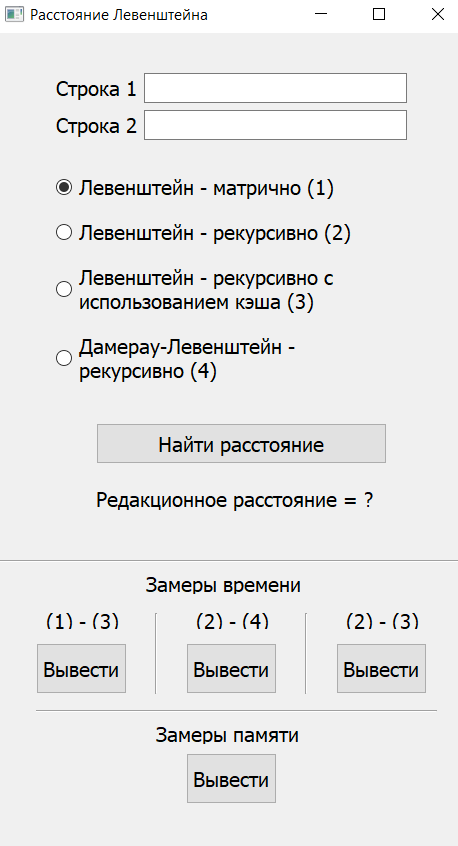
\includegraphics[scale=0.7]{inc/img/interface.png}}
	\caption{Интерфейс программы}
	\label{interface}
\end{figure}

\section{Вывод}
Таким образом, был выбран язык программирования Python для реализации программы, выбраны соответствующие библиотеки, реализованы заданные алгоритмы нахождения расстояний Левенштейна и Дамерау-Левенштейна. Разработан интерфейс, который позволяет пользователю применить каждый из четырех алгоритмов, произвести замеры времени и памяти. 